\section{\color{olive}Excercise 2: Simplification of a Maxterm Expression and its Corresponding Logical Circuit}

Having the function in maxterms $$f_1 (A,B,C,D) = \prod\left(M_0, M_1 , M_5 , M_7 , M_8 , M_{10} , M_{14} , M_{15} \right)$$ equivalent to $$f_2 (A,B,C,D) = \sum\left(m_2, m_3 , m_4 , m_6 , m_9 , m_{11} , m_{12} , m_{13} \right)$$ using minterms, can be simplified by different ways and represented using logic gates.

    \subsection{\color{purple}Simplification by Boolean Algebra}

    The function can be simplified by using the Boolean algebra property (1): $$(A+B).(A+\overline{B})=A~(1)$$ or $$(AB)+(A\overline{B})=A~(2)$$ the function can be simplified using (1):
    \begin{eqnarray*}
        f_1 (A,B,C,D) &= &(A+B+C+D).(A+B+C+\overline{D}).(A+\overline{B}+C+\overline{D}).(A+\overline{B}+\overline{C}+\overline{D}).\\
        &&(\overline{A}+B+C+D).(\overline{A}+B+\overline{C}+D).(\overline{A}+\overline{B}+\overline{C}+D).(\overline{A}+\overline{B}+\overline{C}+\overline{D}) \\
        &=&(A+B+C).(A+\overline{B}+\overline{D}).(\overline{A}+B+D).(\overline{A}+\overline{B}+\overline{C})
    \end{eqnarray*}
    Using the Boolean algebra property (2):
    \begin{eqnarray*}
        f_2(A,B,C,D) &= &(\overline{A}\overline{B}C\overline{D})+(\overline{A}\overline{B}CD)+(\overline{A}B\overline{C}\overline{D})+(\overline{A}BC\overline{D})+\\
        &&(A\overline{B}\overline{C}D)+(A\overline{B}CD)+(AB\overline{C}\overline{D})+(AB\overline{C}D)\\
        &=&(A\overline{B}D)+(\overline{A}B\overline{D})+(\overline{A}\overline{B}C)+(AB\overline{C})
    \end{eqnarray*}

    \subsection{\color{purple}Simplification by Karnaugh Map}

    A Karnaugh map is an easier way to simplify logic expressions when the function is too complex or too large to handle, because the Karnaugh map gives a more representative view for a faster analysis.

    If the simplification is done with minterms, groups are formed by 1's that are together. The ammount of ones that can be present in a group, is a power of two. Each group is represented in the equation by ANDS between the independent variables it contains (the ones that change). The groups are put together by using an OR between them.
    \begin{center}
        \begin{Karnaugh}
            %cada 4 es una fila, la col 3 es la 4ta columna y 3fila es la 4 fila
            \contingut{
            0,1,0,1,
            0,0,1,1,
            1,1,0,0,
            1,0,1,0}
            \implicant{6}{14}{red}
            \implicant{3}{7}{green}
            \implicant{12}{8}{orange}
            \implicantdaltbaix[3pt]{1}{9}{blue}
            %\implicantcantons[2pt]{orange}
            %\implicantcostats{4}{14}{green}
        \end{Karnaugh}
    \end{center}

    Now grouping by colours we get that the function expressed in minterms is:
    \begin{eqnarray*}
        f_2(A,B,C,D)&=&(A\overline{B}D)~(Red)\\
        &&+(\overline{A}B\overline{D})~(Blue)\\
        &&+(\overline{A}\overline{B}C)~(Orange)\\
        &&+(AB\overline{C})~(Green)
    \end{eqnarray*}

    The same method can be done with maxterms; grouping zeroes (instead of ones) in powers of 2, making an AND between groups in case there is more than one, and each group is represented with an OR of its independent variables.

    \subsection{\color{purple}Logic Circuit: AND, OR and NOT}

    Using the logic gates AND, OR and NOT the simplified version of the function could be represented by the figure below:

    \begin{figure}[htb!]
        \centering
        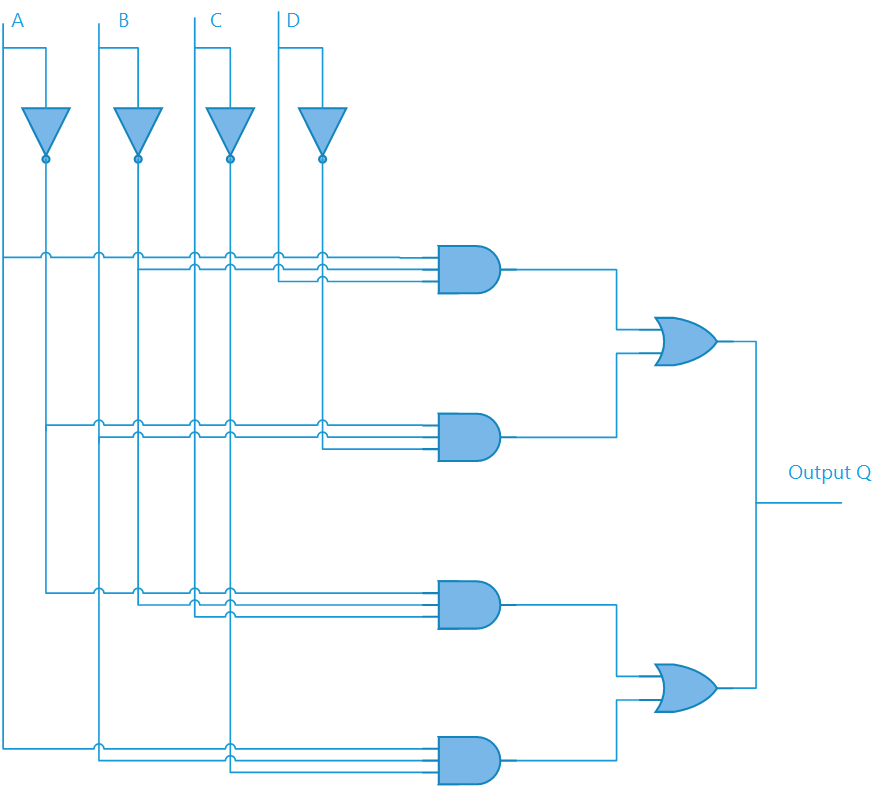
\includegraphics[scale=0.45]{../E2TP1/normallogic.png}
        \caption{\color{cyan}Logic circuit using AND, OR and NOT gates}
        \label{fig:normllogic}
    \end{figure}

    \pagebreak

    \subsection{\color{purple}Logic Circuit: NAND}

    All the gates used above could be equivalent to a combination of NAND or NOR gates. Therefore, the simplified function can be drawn as the next figure:

    \begin{figure}[h!]
        \centering
        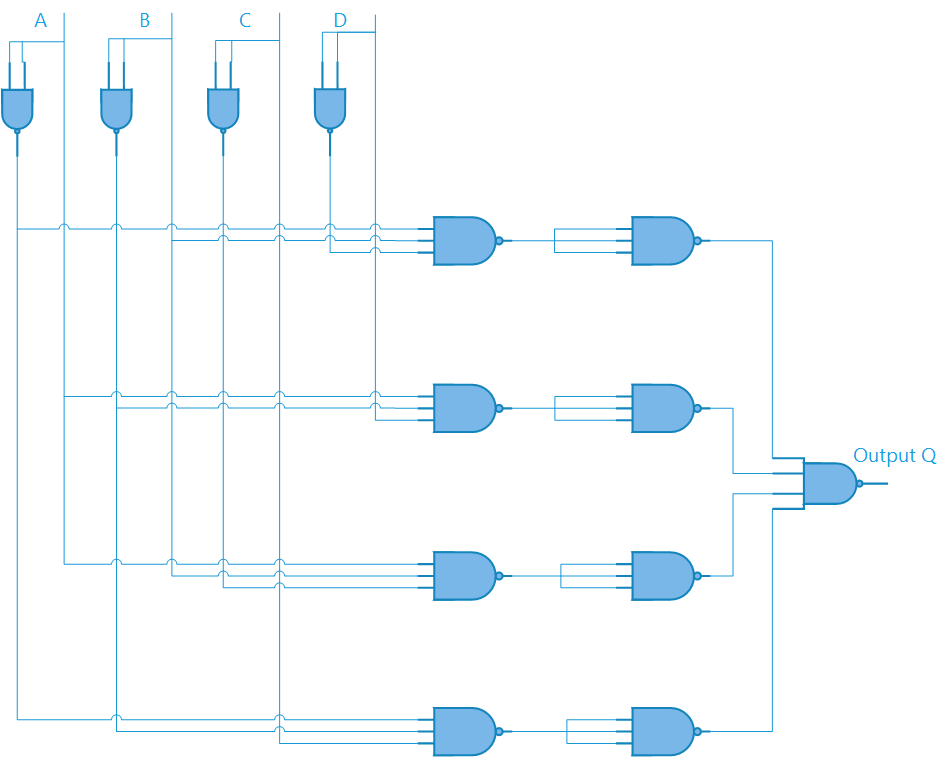
\includegraphics[scale=0.45]{../E2TP1/nandlogic.png}
        \caption{\color{cyan}Logic circuit using NAND gates}
        \label{fig:nandlogic}
    \end{figure}
